\section{Simulación de 5 cuerpos gravitacionales}
Simular el movimiento de 5 cuerpos gravitacionales. Los primeros 4 se ubican
en los vértices de un cuadrado de lado $a$. Encontrar las aceleraciones,
modificar las funciones de dichas aceleraciones y graficar las trayectorias
resultantes.

\subsection{Modelo y aceleraciones}

El sistema consiste en cuatro masas fijas ubicadas en los vértices de un
cuadrado de lado $a = 2$, y una quinta partícula $C_5$ que se mueve libremente
bajo la atracción gravitacional de las cuatro masas. A diferencia del problema
general de $N$ cuerpos, aquí solo $C_5$ se desplaza, mientras que las masas de
los vértices permanecen estáticas.

La aceleración de $C_5$ en la posición $(x, y)$ se obtiene sumando la
contribución gravitacional de cada masa fija:

\begin{equation}
    \vec{a}_5 = \sum_{k=1}^{4} \frac{\vec{r}_k - \vec{r}_5}{|\vec{r}_k - \vec{r}_5|^3}
\end{equation}

donde $\vec{r}_k$ es la posición del vértice $k$ y $\vec{r}_5 = (x, y)$ es la
posición actual de $C_5$. Esta expresión corresponde directamente a la ley de
gravitación de Newton con $G = 1$ y masas unitarias. No se emplea parámetro de
suavizado, por lo que se detecta explícitamente una colisión cuando $C_5$ se
aproxima a menos de $R_\text{col} = 0.5$ de alguna masa fija, descartando esa
trayectoria.

Para explorar distintas trayectorias se realiza un barrido sobre la velocidad
horizontal inicial $v_{x0}$ de $C_5$, manteniendo fijas su posición inicial
$(x_0, y_0) = (2, 7)$ y velocidad vertical $v_{y0} = 0$. De todas las
trayectorias simuladas se seleccionan las cinco cuya trayectoria más se aproxima
al punto de partida, es decir, las más cercanas a ser órbitas cerradas.

\subsection{Implementación}

El primer bloque define los parámetros del sistema: el lado del cuadrado
$a = 2$, el paso de integración $h = 0.01$, el tiempo de simulación
$t_\text{fin} = 750$, las condiciones iniciales de $C_5$ y el barrido de
velocidades $v_{x0} \in [0,\, 1.4]$. También se establecen las posiciones
fijas de los cuatro vértices y el radio de colisión $R_\text{col} = 0.5$.

\inputminted[linenos, frame=lines, fontsize=\footnotesize,
    breaklines=true, firstline=1, lastline=20
]{python}{code/problem03.py}
\inputminted[linenos, frame=lines, fontsize=\footnotesize,
    breaklines=true, firstline=22, lastline=32
]{python}{code/problem03.py}
\captionof{listing}{Parámetros del sistema, condiciones iniciales y posiciones de los vértices.}
\label{lst:prob3_1}

\vspace{10pt}

El segundo bloque define la función \texttt{acel\_cuadrado}, que calcula la
aceleración gravitacional sobre $C_5$ sumando la atracción de cada una de las
cuatro masas fijas. Luego, el bucle principal itera sobre cada valor de
$v_{x0}$, integra la trayectoria mediante el método de Euler, detecta posibles
colisiones y almacena las trayectorias válidas. Al finalizar, se ordenan por
distancia mínima al punto de partida y se seleccionan las cinco más cerradas.

\inputminted[linenos, frame=lines, fontsize=\footnotesize,
    breaklines=true, firstline=34, lastline=55
]{python}{code/problem03.py}
\inputminted[linenos, frame=lines, fontsize=\footnotesize,
    breaklines=true, firstline=57, lastline=95
]{python}{code/problem03.py}
\captionof{listing}{Función de aceleración gravitacional, integración por Euler y selección de trayectorias.}
\label{lst:prob3_2}

\vspace{10pt}

El tercer bloque genera la figura con fondo oscuro. Cada trayectoria
seleccionada se traza con un color distinto e incluye su valor de $v_{x0}$ en
la leyenda. Las cuatro masas fijas se representan como círculos rellenos en los
vértices del cuadrado, unidos por un contorno punteado, y $C_5$ aparece como un
círculo blanco en el origen para referencia visual.

\inputminted[linenos, frame=lines, fontsize=\footnotesize,
    breaklines=true, firstline=97, lastline=145
]{python}{code/problem03.py}
\captionof{listing}{Configuración visual y generación de la figura de trayectorias.}
\label{lst:prob3_3}

\vspace{10pt}

La Figura \ref{fig:prob3_1} muestra las cinco trayectorias más cerradas
obtenidas para $C_5$ durante el tiempo de simulación $t_\text{fin} = 750$.

\begin{figure}[H]
  \centering
  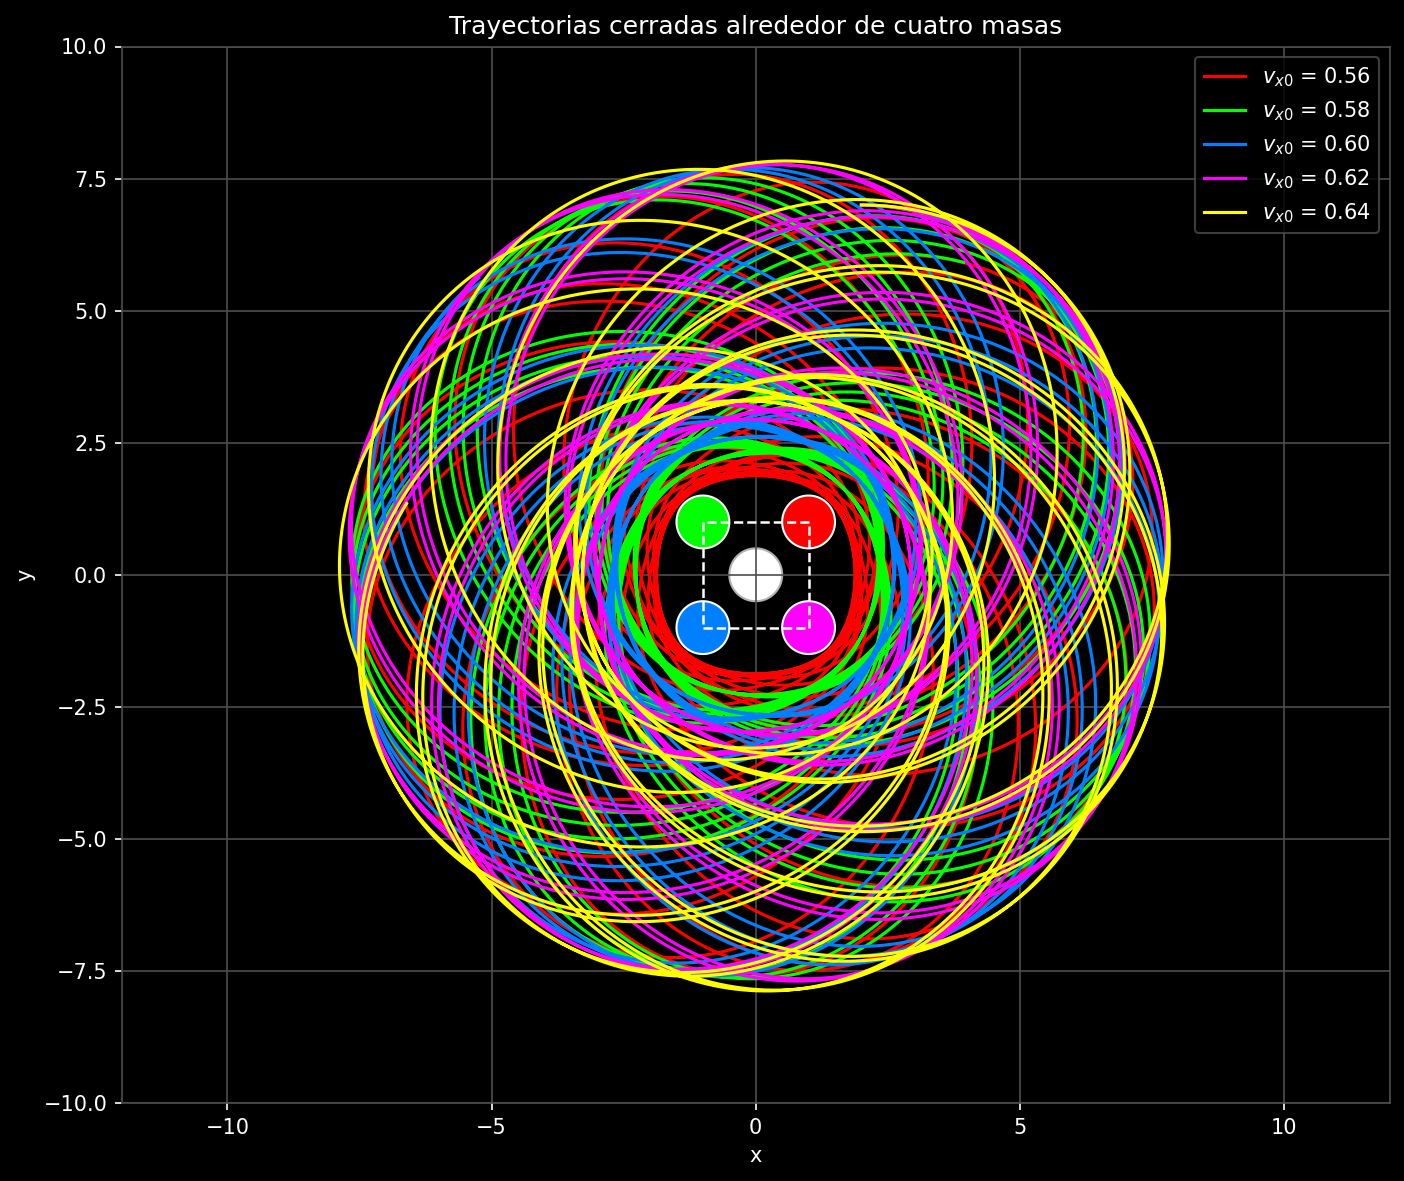
\includegraphics[width=1.0\textwidth]{images/problem03.png}
  \caption{Trayectorias de $C_5$ bajo la atracción de cuatro masas fijas en los
  vértices del cuadrado. Se muestran las cinco órbitas cuya trayectoria más se
  aproxima al punto de partida.}
  \label{fig:prob3_1}
\end{figure}

\vspace{10pt}

Se observa que $C_5$ describe trayectorias complejas bajo la influencia
simultánea de las cuatro masas fijas. Ninguna de las órbitas obtenidas es
perfectamente cerrada, pero las seleccionadas presentan el mayor grado de
recurrencia al punto de partida. La simetría del cuadrado impone cierta
regularidad en las trayectorias, que tienden a rodear el conjunto de masas o a
oscilar entre ellas. La velocidad inicial $v_{x0}$ determina si $C_5$ escapa
hacia el exterior, queda atrapada en una órbita acotada o impacta contra alguna
de las masas.

\subsection{Conclusión}

La simulación reproduce la dinámica gravitacional de una partícula bajo la
atracción de cuatro masas fijas mediante la ley de gravitación de Newton. Las
trayectorias obtenidas muestran que la geometría del cuadrado genera un campo
gravitacional con simetría cuadrada que atrapa a $C_5$ en órbitas complejas
para ciertos valores de $v_{x0}$. El método de Euler permite integrar el
sistema de forma sencilla, aunque acumula error con el tiempo, lo que limita la
precisión de las trayectorias para simulaciones largas.